Dans ce chapitre, nous abordons plusieurs méthodes de simulation de variables aléatoires. 

\vspace{\baselineskip}
Pour une loi de probabilité donnée (par exemple, la loi normale), le calcul de probabilités permet de calculer des quantités associées, telles que l'espérance, la variance, la fonction de répartition.
Cependant, peut on définir une méthode algorithmique permettant de générer un échantillon aléatoire issu de cette loi? 
C'est à dire une suite de variable aléatoires $X_1, \dots, X_n$ telles qu'elles soient mutuellement indépendantes, et distribuées selon cette loi?

En pratique, il n'existe pas aujourd'hui de méthode générique de simulation \textit{aléatoire}\footnote{Au sens commun du terme, c'est à dire \textit{imprévisible} exactement par quiconque} par ordinateur. 
Cependant, des algorithmes \textit{déterministes} ont été proposés pour \textit{mimer} un comportement de variables aléatoires indépendantes et identiquement distribuées. 
Ces algorithmes sont appelés \textit{générateurs pseudo-aléatoires}. 
En pratique, la simulation d'une variable aléatoire de loi quelconque se ramènera de manière "atomique" à la simulation d'une loi uniforme sur l'intervalle $[0, 1]$ \footnote{Autrement dit, toute quantité aléatoire utilisée sera algorithmiquement obtenue à partir de transformation déterministes de lois uniformes.}. 
On décrira donc dans la section suivante un générateur pseudo aléatoire pour la loi uniforme sur $[0, 1]$.

\subsection{Générateur à congruences pour la loi $\Unif[0,1]$}
\label{sec:gen:unif}
Dans cette section, on présente un algorithme déterministe de simulation pour simuler une loi uniforme sur l'intervalle $[0,1]$. Le but de ce polycopié n'est pas de couvrir le très vaste sujet des générateurs pseudos aléatoires. Le lecteur intéressé pourra se référer au chapitre 3 de \cite{knuth1997art}. Les notations de cette section sont d'ailleurs issues de cette référence.

\vspace{\baselineskip}
\textbf{Algorithme} Une méthode générique pour mimer le comportement d'un échantillon de variables aléatoires $U_1, \dots, U_n$ indépendantes et identiquement distribuées de loi $\Unif[0,1]$ la méthode de congruence linéaire.

L'algorithme se base sur 4 données initiales choisies par l'utilisateur:
\begin{itemize}
\item Un entier $m > 0$, appelé \textit{module};
\item Un entier $0 < a < m$  appelé \textit{multiplicateur};
\item Un entier $0 \leq c < m$ appelé \textit{incrément};
\item Un entier $0 \leq x_0 < m$ appelé \textit{graine}.
\end{itemize}
On créera alors une suite de nombres $x_1,\dots x_n$ en utilisant la relation de récurrence
\begin{align*}
x_k = = (a x_{k-1} + c) \text{ modulo }m. 
\end{align*}
On définit enfin les nombres $u_1,\dots,u_n$ tels que $u_k = \frac{x_k}{m},~1\leq k \leq n$, qui sont, par construction, dans l'intervalle $[0, 1]$. La méthode est entièrement résumé par l'Algorithme \ref{alg:GenCong}. 
%%%%%%%%%%%%%%%%%%%%%%%%%%%%%%%%%
\IncMargin{1em}
\begin{algorithm}[h]
\caption{\label{alg:GenCong} Générateur à congruences}
\SetKwInOut{Input}{Entrée}
\SetKwInOut{Output}{Sortie}
\Input{5 entiers $m$, $a$, $c$, $x_0$ et $n$}
\Output{$u_1,\dots,u_n$: réalisation pseudo-aléatoire d'un échantillon i.i.d. de loi $\Unif[0,1]$}
\BlankLine
\For{$k\leftarrow 1$ \KwTo $n$}
{$x_k \leftarrow (a x_{k-1} + c) \text{ modulo } m$\;
$u_k \leftarrow x_k / m$\;
}
\end{algorithm}
\DecMargin{1em}
%%%%%%%%%%%%%%%%%%%%%%%%%%%%%%%%%

\vspace{\baselineskip}
La séquence $u_1,\dots,u_n$ ainsi générée est donc à valeurs dans $[0, 1]$ \footnote{Plus exactement dans $[0, 1[$ telle que définie ici. Si on prend $c = 0$ et $m$ premier, elle est même à valeurs dans $]0, 1[$.}. 
Pour des valeurs de $a, c$ et $m$ bien choisies, cette séquence se comporte comme la réalisation d'un échantillon de $n$ variables aléatoires $U_1,\dots, U_n$ indépendantes et identiquement distribuées de loi $\mathcal{U}[0 , 1]$.

Un générateur à congruences correspond au choix de $a, c$ et $m$.
La graine $x_0$ correspond au point de départ de l'algorithme. 
Pour un $x_0$ fixé, la séquence obtenue en sortie sera \textit{toujours} la même. 
En pratique, quand un tel algorithme est appelé dans un ordinateur, la graine n'est pas demandée à l'utilisateur, mais obtenue en interne. 
Une méthode générique est de prendre le nombre de millisecondes (modulo $m$) écoulé depuis le 1er Janvier 1970.

\vspace{\baselineskip}
\textbf{Choix de $a$, $c$ et $m$:} Le choix des constantes du générateur est une question délicate. 

Un premier point important est que la "loi" de l'échantillon obtenu doit mimer celle de la loi cible. 
Pour ce faire, on pourra utiliser un test statistique (voir la section \ref{sec:test:adequation}.

Un autre point est que l'échantillon simuler doit mimer l'indépendance. 
Or, il faut d'ores et déjà remarquer que chaque $x_k$ est dans l'ensemble fini $\left\lbrace 0,\dots, m-1\right\rbrace$, ainsi, la suite $(x_n)_{n\geq 0}$ est nécessairement \textit{périodique}.

Un facteur souhaité pour mimer l'aléatoire est que cette période ne soit pas "visible" par l'utilisateur, ainsi on voudra qu'elle soit longue, ce qui implique que $m$ soit grand. De même, pour que la période soit grande, il faut en pratique que $a$ soit grand, et, si possible, relativement premier à $m$.
Un autre aspect pris en compte doit être la rapidité de l'opération "modulo $m$". 
Nous n'irons pas plus point concernant ces points, largement discutés dans \citep{knuth1997art}. 
Un tableau des valeurs utilisées pour les générateurs les plus connus et disponible dans le chapitre 1 de \citep{delyon2017simulation}.

\vspace{\baselineskip}
Dans la suite du cours, on supposera que l'on dispose d'une méthode valide de simulation de variables uniformes indépendantes. 
La plupart des langages informatiques en dispose. 
Dans le logiciel \texttt{R}, cette méthode est implémentée dans la fonction \texttt{runif}. 

\subsection{Méthodes de simulation de lois} 

On s'intéresse désormais à simuler une variable aléatoire quelconque.

\subsubsection{Rappels sur la fonction de répartition}

\begin{definition}{\textit{Fonction de répartition}}
Soit $X$ une variable aléatoire à valeurs réelles. Pour tout réel $x$, on appelle fonction de répartition de $X$ la fonction $F_X$:
\begin{align*}
\begin{array}{ccl}
\R &\mapsto& [0, 1]\\
x &\mapsto& F_X(x) = \mathbb{P}(X \leq x)
\end{array}
\end{align*}
Une fonction de répartition $F_X$ est caractérisée par les propriétés suivantes:
\begin{enumerate}
\item $F_X$ est partout continue à droite, i.e. pour tout $x\in \R$: $$\lim_{h \underset{>0}{\rightarrow} 0} F(x + h) = F(x)$$
\item $F_X$ est croissante.
\item $\lim_{x \rightarrow -\infty}F_X(x) = 0, \lim_{x \rightarrow +\infty}F_X(x) = 1$
\end{enumerate}
Ainsi, toute fonction $F$ sur $\R$ satisfaisant ces conditions est une fonction de répartition.

Des exemples de fonctions de répartitions sont montrés sur la Figure \ref{fig:fonc:rep}.
\end{definition}
\begin{figure}[ht]
\centering
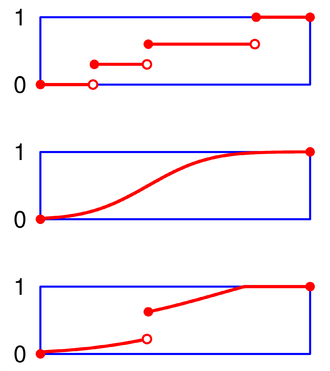
\includegraphics[height = 0.3\textheight]{figures/fonction_repartition}
\caption{\label{fig:fonc:rep} Exemples de fonction de répartition pour une variable aléatoire discrète (haut), continue (centre) ou avec atome (bas). Source \textit{Wikipedia}.}
\end{figure}

Une fonction importante définie à partir de la fonction de répartition est son inverse généralisée. 
Cette fonction est l'outil de la base de la méthode d'inversion décrite plus bas.

\begin{definition}{\textit{Inverse généralisée}}
Soit $F$ une fonction de répartition, on appelle inverse généralisée de $F$, notée, $F^{-1}$ la fonction:
\begin{align*}
\begin{array}{ccl}
]0, 1[&\mapsto& \R\\
u &\mapsto& F^{-1}(u) = \inf\left\lbrace z \in \R \text{ tel que } F(z) \geq u \right\rbrace
\end{array}
\end{align*}
Pour une variable aléatoire $X$, la fonction $F_X^{-1}$ est également appelée \textit{fonction quantile} de la variable aléatoire $X$.
Dans ce cas, on convient que $F_X^{-1}(0)$ et $F_X^{-1}(1)$ sont  la plus petite et la plus grande des valeurs possibles pour $X$ (éventuellement infinies).
\end{definition}

\vspace{\baselineskip}
\textbf{Remarque:} Dans le cas d'une fonction de répartition $F$ continue et strictement croissante sur $\R$\footnote{Associée à une variable aléatoire continue sur $\R$, par exemple}, la fonction $F^{-1}$ est simplement l'inverse de $F$.

\begin{definition}{\textit{Fonction de répartition empirique}}

Soit $X_1, \dots, X_n$ un échantillon de variables aléatoires indépendantes et identiquement distribuées selon la loi d'une variable aléatoire $X$.

La fonction de répartition empirique de la variable aléatoire $X$ associée à $X_1,\dots X_n$, notée $F_X^n$ est la fonction:
\[
\begin{array}{ccl}
\R &\mapsto& [0, 1]\\
x &\mapsto& F_X^n(x) = \frac{1}{n}\underset{i=1}{\overset{n}{\sum}} \mathbf{1}_{X_i \leq x}
\end{array}
\]
On vérifie facilement que $F^n_X$ est une fonction de répartition.
\end{definition}


\subsubsection{Méthode d'inversion}

Supposons qu'on connaisse la fonction de répartition de $X$, $F_X$, alors on a la propriété suivante (propriété d'inversion):

\begin{propriete}{\textit{Méthode d'inversion}}\label{prop:meth:inv}

Soit $F$ une fonction de répartition. Soit $F^{-1}$ son inverse généralisée. Soit $U$ une variable aléatoire de loi uniforme sur $[0, 1]$, alors la variable aléatoire $$X := F^{-1}(U)$$ admet $F$ comme fonction de répartition.
\end{propriete}

\begin{proof}
On veut montrer que, pour tout $x\in \R$ 
\begin{align*}
\mathbb{P}(F^{-1}(U) \leq x) &= F(x).
\intertext{Montrons tout d'abord que, pour tout $u \in ]0, 1[$}
\forall x \in \R,F^{-1}(u) \leq x &\Leftrightarrow u \leq F(x).
\end{align*}
\begin{itemize}
\item[$\Rightarrow$] Soient $u \in ]0, 1[$ et $x\in \R$ tels que $F^{-1}(u) \leq x$. \newline
Par croissance de $F$, on a donc:
\begin{align*}
F\left(F^{-1}(u)\right) &\leq F(x)
\intertext{Or, en se souvenant que par définition}
F^{-1}(u) &= \inf\left\lbrace z \in \R \text{ tel que } F(z) \geq u \right\rbrace,
\intertext{on a donc directement}
u&\leq  F\left(F^{-1}(u)\right) \leq F(x)
\end{align*}
\item[$\Leftarrow$] Soient $u \in ]0, 1[$ et $x\in \R$ tels que $u \leq F(x)$.\newline
Ainsi, $x\in\left\lbrace z \in \R \text{ tel que } F(z) \geq u \right\rbrace$, donc $F^{-1}(u) \leq x$.
\end{itemize}
On a donc montré, l'équivalence. 
Il reste à conclure en se servant de la définition d'une loi uniforme:
$$\mathbb{P}(F^{-1}(U) \leq x) = \mathbb{P}(U \leq F(x))  = F(x).$$
\end{proof}

\textbf{Conséquence et intérêt de la Proposition \ref{prop:meth:inv}:} Comme conséquence immédiate de cette proposition, on obtient une méthode de simulation d'un échantillon pour une variable aléatoire $X$ de loi de probabilité $F_X$:
\begin{enumerate}
\item Calculer $F^{-1}_X$
\item Simuler un échantillon aléatoire i.i.d. $U_1,\dots,U_n$de loi $\Unif[0,1]$\footnote{Qu'on est capable de simuler grâce à un algorithme similaire à ceux décrit en \ref{sec:gen:unif}.}
\item Obtenir un échantillon i.i.d. $X_1,\dots,X_n = F_X^{-1}(U_1),\dots, F_X^{-1}(U_n)$
\end{enumerate} 

\subsubsection{Méthode d'acceptation rejet}

La méthode d'acceptation rejet permet de simuler selon une densité $f$, évaluable en tout point, même lorsque la méthode d'inversion ne peut être appliquée.

L'idée est de se servir d'une loi qu'on sait simuler (la loi de proposition), de densité $g$, et ayant un support couvrant celui de $f$.

\begin{propriete}{\textit{Méthode d'acceptation-rejet}}\label{prop:meth:ar}
Soit $f$ et $g$ deux densités sur $\R^d$.
On suppose qu'il existe une constante $M$ telle que 
$$\forall x \in \R~~f(x) \leq M(g(x))$$
On note 
$$\alpha(x) := \frac{f(x)}{Mg(x)}.$$
Soit $(U_n)_{n\geq 1}$ une suite de variables aléatoires i.i.d. de loi uniforme sur $[0, 1]$. Soit $(Y_n)_{n\geq 1}$ une suite de variables aléatoires i.i.d. de densité $g$.
On note $T$ la variable aléatoire (à valeurs dans $\mathbb{N}^*$):
$$T = \inf\left\lbrace n, \text{ tel que } U_n \leq \alpha(Y_n)\right\rbrace.$$.
Alors, la variable aléatoire $X := Y_T$ ($T$-ième valeur de la suite  $(Y_n)_{n\geq 1}$ a pour densité $f$).
\end{propriete}

\begin{proof}
Soit un entier $n\leq 1$:
\begin{align*}
\mathbb{P}\left(X\leq x, T = n \right) &=  \mathbb{P}\left( U_1 > \alpha(Y_1), \dots, U_{n - 1} > \alpha(Y_{n-1}), U_n \leq \alpha(Y_n), Y_n \leq x  \right)
\intertext{Par propriété d'indépendance}
&= \mathbb{P}\left(U_n \leq \alpha(Y_n), Y_n \leq x  \right)\prod_{i = 1}^{n-1}\mathbb{P}\left(U_i > \alpha(Y_i)\right)
\intertext{Par propriété de distribution identique}
&= \mathbb{P}\left(U_n \leq \alpha(Y_n), Y_n \leq x  \right)\mathbb{P}\left(U_1 > \alpha(Y_1)\right)^{n-1}
%%%%%% PREMIER TERME%%%%
\intertext{Or on a:}
\mathbb{P}\left(U_1 > \alpha(Y_1)\right) &= \E\left[\mathbf{1}_{U_1 > \alpha(Y_1)}\right]\\
&= \int_{\R} \left(\int_0^1 \mathbf{1}_{u > \frac{f(y)}{Mg(y)}} \rmd  u\right)\times g(y) \rmd y\\
&=\int_{\R} (1 -  \frac{f(y)}{Mg(y)})g(y) \rmd y
\intertext{Comme $f$ et $g$ sont des densités:}
\mathbb{P}\left(U_1 > \alpha(Y_1)\right) &=1 - \frac{1}{M}
\intertext{De manière analogue}
\mathbb{P}\left(U_n \leq \alpha(Y_n), Y_n \leq x  \right) &= \E\left[\mathbf{1}_{U_n \leq \alpha(Y_n)}\times \mathbf{1}_{Y_n \leq x}\right]\\
&=  \int_{\R} \left(\int_0^1 \mathbf{1}_{u \leq \frac{f(y)}{Mg(y)}} \rmd  u\right)\times \mathbf{1}_{y \leq x} g(y) \rmd y\\
&= \int_{-\infty}^x \frac{f(y)}{M}\rmd y\\
&= \frac{F(x)}{M},
\intertext{où $F(x)$ est la fonction de répartition associée à $f$. En résumé:}
\mathbb{P}\left(X\leq x, T = n \right) &= \frac{F(x)}{M}\left(1 - \frac{1}{M}\right)^{n - 1}
\end{align*}
Donc on conclut en remarquant que  
$$\mathbb{P}(X\leq x) = \sum_{n = 1}^\infty \mathbb{P}\left(X\leq x, T = n \right) = F(x)$$
\end{proof}

\vspace{\baselineskip}
\textbf{Remarque sur la loi du temps d'attente:} De la preuve, on peut déduire que 
$$\mathbb{P}\left(T = n \right) = \lim_{x \rightarrow \infty}\mathbb{P}\left(X\leq x, T = n \right) = \lim_{x \rightarrow \infty} \frac{F(x)}{M}\left(1 - \frac{1}{M}\right)^{n - 1} =  \frac{1}{M}\left(1 - \frac{1}{M}\right)^{n - 1}$$
Donc, la loi du temps d'attente avant d'obtenir une réalisation de $F$ est une loi géométrique de paramètre $\frac{1}{M}$. 

L'espérance du nombre d'essais avant le premier succès est donc $M$. 

Pour un $g$ donné, l'algorithme est optimal en complexité quand $M$ est minimal.

\vspace{\baselineskip}
\textbf{Cas de lois discrètes} La proposition \ref{prop:meth:ar:disc} permet de simuler pour des variables aléatoires à densité. Un analogue existe pour les variables aléatoires discrètes.

\begin{propriete}{\textit{Méthode d'acceptation-rejet, cas discret}}\label{prop:meth:ar:disc}
Soit $X$ une variable aléatoire discrète sur l'ensemble $\left\lbrace 1,\dots, K\right\rbrace$ et $Y$ une variable aléatoire discrète sur l'ensemble $\left\lbrace 1,\dots, K'\right\rbrace$ (avec $K' \geq K$).
On suppose qu'il existe une constante $M$ telle que 
$$\forall k \in \left\lbrace 1,\dots, K'\right\rbrace~~\mathbb{P}(X = k) \leq M\mathbb{P}(Y=k)$$
On note 
$$\alpha(k) := \frac{\mathbb{P}(X = k)}{M\mathbb{P}(Y=k)}.$$
Soit $(U_n)_{n\geq 1}$ une suite de variables aléatoires i.i.d. de loi uniforme sur $[0, 1]$. Soit $(Y_n)_{n\geq 1}$ une suite de variables aléatoires i.i.d. de même loi que $Y$.
On note $T$ la variable aléatoire (à valeurs dans $\mathbb{N}^*$):
$$T = \inf\left\lbrace n, \text{ tel que } U_n \leq \alpha(Y_n)\right\rbrace.$$
Alors, la variable aléatoire $Y_T$ ($T$-ième valeur de la suite  $(Y_n)_{n\geq 1}$ a la même loi que $X$.
\end{propriete}

\begin{proof}
La preuve est l'analogue pour les lois discrètes de la précédente.
\end{proof}

\subsubsection{Utilisation de transformation usuelles}

On peut bien évidemment utiliser la théorie des probabilités pour simuler différentes lois, notamment les règles sur la stabilité des lois:

\begin{itemize}
\item Si $c > 0$ et $d\in\mathbb{R}$ $U \sim \Unif[a, b] \Rightarrow cU + d \sim \Unif[ac + d, bc + d]$
\item Si $X\sim\Nor (\mu, \sigma^2) \Rightarrow aX +b \sim \Nor(a\mu + b, a^2\sigma^2)$
\item Etc...
\end{itemize}

\subsection{Vecteurs aléatoires}

Supposons qu'on veuille simuler un vecteur aléatoire (X, Y) où $X$ et $Y$ sont deux variables aléatoires réelles (cela s'étend évidemment à un vecteur de taille $n$). 

Un cas simple est quand $X$ et $Y$ sont indépendantes, alors, on se ramène au cas univarié, et le couple aléatoire est donné par deux réalisations indépendantes.

Dans les autres cas, certaines méthodes peuvent s'avérer utiles.

\subsubsection{Conditionnement}

Un cas utile en pratique est le cas où l'on sait simuler facilement $X$, et l'on sait facilement simuler $Y$ sachant $X$. 

On utilise alors la décomposition de la loi jointe

$$\Pro(X\leq x, Y\leq y) = \Pro(Y\leq y \vert X\leq x) \times \Pro(X\leq x)$$

\textbf{Exemple} Supposons qu'on veuille simuler selon la densité jointe:
$$f_{X,Y}(x, y) = x\e{-xy}\I{0\leq x\leq 1}\I{y>0}$$
Alors, la densité marginale de $X$ est donnée par:
$$f_X(x) = \int_0^\infty x\e{-xy}\I{0\leq x\leq 1}\rmd y = \I{0\leq x\leq 1}$$
Ainsi, $X$ suit une loi uniforme sur $[0, 1]$. $x$ étant fixé, la loi de $Y\vert X$ est donnée par une loi exponentielle de paramètre $x$. On peut donc facilement simuler $(X, Y)$ en simulant selon une uniforme, puis une exponentielle de paramètre donné par cette uniforme.

\subsubsection{Changement de variables}

Pour les couples de variables aléatoires à densité, on peut utiliser la propriété du changement de variables. 
\begin{propriete}
Soit un couple de variables aléatoires $(U,V)$ de densité $f_{U,V}(u,v)$ définie sur $E_{UV} \subset \R^2$ et un couple de variables aléatoires $(X, Y)$ à valeurs dans $E_{XY} \subset \R^2$. Supposons qu'il existe une application $\phi$, $C^1$, inversible, et d'inverse $C_1$, tel que $(X, Y) = \phi(U, V)$, alors la densité jointe de $(X, Y)$ est donnée par:
$$f_{X,Y}(x, y) = f_{U,V}(\phi^{-1}(x, y))\vert\det J_{\phi^{-1}}(x, y)\vert  $$
\end{propriete}
où $J_\phi$ désigne la matrice jacobienne d'une application $\phi(u, v)$:
$$J_\phi(u, v) = \begin{pmatrix}
\frac{\delta \phi_1}{\delta u}(u, v) & \frac{\delta \phi_1}{\delta v}(u, v)\\
\frac{\delta \phi_2}{\delta u}(u, v) & \frac{\delta \phi_2}{\delta v}(u, v)
\end{pmatrix}$$

\subsubsection{Simulation d'un vecteur Gaussien}
En pratique, un type de vecteur aléatoire important est le vecteur Gaussien.
En dimension $d$, un vecteur Gaussien $X = \left(X_1,\dots,X_d\right)'$ est un vecteur dont toutes les combinaisons linéaires des composantes sont des lois Gaussiennes sur $\R$.

Il est entièrement caractérisé par le vecteur $\E[X] = \left(E[X_1], \dots, \E[X_d]\right)'$ et sa matrice de variance (covariance) $\Sigma$:
$$\Sigma_{i,j} = \Cov[X_i, X_j]$$
Il se trouve qu'un vecteur Gaussien est stable par transformation affine.

Ainsi, si $X$ est un vecteur Gaussien de paramètres $\mu := \E[X]$ et de variance $\Sigma$, alors pour un vecteur $b$ de taille $d$ et une matrice $d \times d$, alors $$AX + b \sim \Nor(A\mu + b, A\Sigma A').$$
Cette propriété implique qu'on peut simuler tout vecteur Gaussien à partir de $d$ variables aléatoires Gaussiennes indépendantes centrées et réduites. 
Pour une matrice de variance $\Sigma$ voulu, il suffit de trouver $R$ tel que $RR' = \Sigma$. Ce calcul est toujours possible car $\Sigma$ est une matrice semi-définie positive. 

\subsection{Complément: Test statistique d'adéquation à une loi}
\label{sec:test:adequation}

Dans ce chapitre, nous avons défini des algorithmes de simulation  d'échantillons aléatoires. 

Correctement évaluer si un algorithme reproduit un comportement aléatoire est un sujet très vaste en informatique, qui ne sera pas abordé ici (encore une fois, voir \cite{knuth1997art}, ou encore, \citep{cover2006elements}, chapitre 7 sur la théorie de la complexité).

D'un point de vue statistique, la question d'évaluer si un échantillon observé est la réalisation d'un échantillon aléatoire de loi connue est également un problème d'intérêt.

Ce problème peut être traité par différents tests statistiques.
Nous en présenterons ici 2: 
\begin{itemize}
\item Le test du $\chi^2$ d'adéquation (pour l'adéquation a une loi discrète); 
\item Le test de Kolmogorov-Smirnoff, pour l'adéquation a une loi continue
\end{itemize}

\subsubsection{Test du $\chi^2$ d'adéquation}

Le test du $\chi^2$ d'adéquation à une loi permet de tester si un échantillon i.i.d. de v.a. discrètes $X_1,\dots, X_n$, à valeurs dans l'ensemble $\lbrace 1,\dots, K\rbrace$ est distribuée selon une loi multinomiale de paramètre $p^* = (p_1,\dots ,p_K)$.

On définit $N_k = \sum_{i = 1}^n \mathbf{1}_{X_i = k}$ et la variable aléatoire
$$T_n = \sum_{k = 1}^K\frac{(N_k - np_k)^2}{np_k}$$
\paragraph{Propriété: }Quand $n\mapsto \infty$, $T_n$ converge en loi vers un $\chi^2(K - 1)$.
\medskip

Pour le test:
\begin{itemize}
\item[$H_0$] La loi de $X_1$ est $p^*$;
\item[$H_1$] La loi de $X_1$ n'est pas $p^*$,
\end{itemize}
On utilisera $T_n$ comme statistique de test.

Pour un risque de première espèce $\alpha \in ]0, 1[$, 
on aura alors la procédure de test suivante, 

Pour un échantillon observé $x_1,\dots, x_n$, on définit $n_k =  \sum_{i = 1}^n \mathbf{1}_{x_i = k}$. On calcule 
$t_n = \sum_{k = 1}^K\frac{(n_k - np_k)^2}{np_k}$
On rejette alors $H_0$ au risque $\alpha$ si $t_n > z_{1 - \alpha}$ ou $z_{1 - \alpha}$ est le quantile d'ordre 1 - $\alpha$ d'une loi du $\chi^2(n-1)$. 


\subsubsection{Test de Kolmogorov-Smirnoff}

Le test de Kolmogorov-Smirnoff permet de tester l'adéquation échantillon i.i.d. de v.a. continues $X_1,\dots, X_n$ à une loi continue de fonction de répartition $F^*$.

On définit la variable aléatoire
$$T_n = \sqrt{n} \max_{i = 1\dots, n} \vert F_n(X_i) - F(X_i)\vert$$

\textbf{Propriété: }Quand $n\mapsto \infty$, $T_n$ converge en loi vers la variable aléatoire $T$ de fonction de répartition $F_T:$
$$F_T(x) = \left\lbrace 
\begin{array}{lr}
0 & \text{ si } x\leq 0\\
1 - 2 \sum_{k = 1} (-1)^{k + 1} \exp\left(-2 k^2 x^2 \right)& \text{ sinon}
\end{array}
\right.$$
Cette loi est appelée loi de Kolmogorov Smirnoff.


Pour un risque de première espèce $\alpha \in ]0, 1[$, 
on aura alors la procédure de test suivante, 

Pour le test:
\begin{itemize}
\item[$H_0$] La loi de $X_1$ est $F^*$;
\item[$H_1$] La loi de $X_1$ n'est pas $F^*$,
\end{itemize}
On utilisera $T_n$ comme statistique de test.

Pour un échantillon observé $x_1,\dots, x_n$, on calcule la fonction de répartition empirique associée $F_n$ et le $t_n$ correspondant.

On rejette alors $H_0$ au risque $\alpha$ si $1 - F_T(t_n) > 1- \alpha$
\medskip

Ces deux tests peuvent être utiles pour vérifier qu'une méthode de simulation fonctionne.

Nous allons maintenant nous intéresser aux méthodes de simulation proprement dites.
